\section{Modello e implementazione del sistema}\label{sec:modello}
\subsection{Modello del sistema}\label{subsec:modello-del-sistema}
Il sistema del pendolo invertito è riassunto in figura \ref{fig:sistema}.
In questa sezione, ricaverò le equazioni del moto e le linearizzerò attorno al punto di equilibrio instabile.

\begin{figure}[h]
    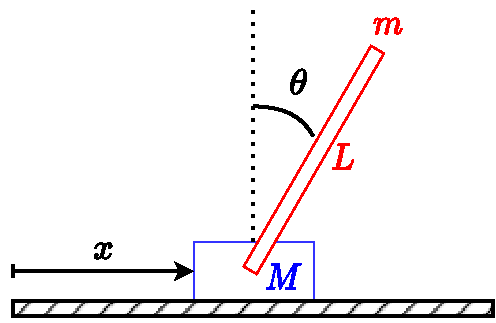
\includegraphics{../assets/sistema.pdf}
  \caption{\emph{Pendolo invertito. Le variabili generalizzate sono $x$ e $\theta$. Il carrello ha massa $M$,
  il pendolo ha lunghezza $L$ e massa $m$. Un motore (non rappresentato in figura) esercita una forza che agisce
  lungo $\hat x$. Si noti che la variabile generalizzata $x$ e lo stato del sistema $\bf x$ sono due grandezze diverse.}}
  \label{fig:sistema}
\end{figure}


La Lagrangiana del sistema è\footnote{Per semplificare i calcoli, avrei potuto scrivere direttamente la Lagrangiana delle
piccole oscillazioni attorno al punto di equilibrio instabile, ottenendo lo stesso risultato. Facendo così, però, non avrei
ottenuto le equazioni non lineari del moto, che mi sono servite per simulare il sistema a computer.}
\begin{equation}
  \begin{aligned}
    \mathcal L &= T - V\\
      &= \frac 1 2 \left[
        M \dot x^2 + mv_{p}^2 + I_{p} \dot \theta^2
      \right] -\\
      &- mg\frac L 2\cos{\theta}
    \end{aligned}
  \label{eq:lagrangiana}
\end{equation}
dove $v_p$ e $I_p$ indicano rispettivamente velocità del centro di massa e momento d'inerzia calcolato rispetto al
centro di massa del pendolo.
In particolare, valgono:
\begin{equation}
  \begin{aligned}
    v_p^2 &= \left(\dot x + \frac L 2 \dot \theta \cos{\theta}\right)^2 + \left(\frac L 2 \dot \theta \sin{\theta}\right)^2 \\
    I_p &= \frac 1 {12} m L^2
  \end{aligned}
  \label{eq:lagrangiana-2}
\end{equation}

Imposto e risolvo le equazioni di Eulero:
\begin{equation}
  \left\{
    \begin{aligned}
      \frac d {dt} \frac {\partial \mathcal L} {\partial \dot x } - \frac {\partial \mathcal L} {\partial  x}&= f \\
      \frac d {dt} \frac {\partial \mathcal L} {\partial \dot \theta } - \frac {\partial \mathcal L} {\partial \theta}&= 0
    \end{aligned}
  \right.
  \label{eq:eulero}
\end{equation}

In questo modo trovo le equazioni del moto non lineari:
\begin{equation}
  \left\{
  \begin{aligned}
    \ddot x &= \frac{2m\sin\theta\left(3g\cos\theta-2l\dot \theta^2\right)-8f}{3m\cos(2\theta)-5m-8M} \\
    \ddot \theta &= \frac{3\sin\theta \left(lm\dot \theta^2\cos\theta-2g(m+M)\right)+6f\cos\theta}{l\left(3m\cos^2\theta-4(m+M)\right)}
  \end{aligned}
  \right.
  \label{eq:moto}
\end{equation}

Ora faccio un cambio di variabile, in modo da avere un sistema di primo ordine.
Ho usato il simbolo $(\ldots)$ al posto di riscrivere le equazioni \eqref{eq:moto} nel sistema.
\begin{equation}
  \dot {\mathbf x} = \left(
  \begin{matrix}
    \dot x \\
    \dot v \\
    \dot \theta \\
    \dot \omega
  \end{matrix}\right) = \left(
  \begin{matrix}
    v \\
    (\ldots) \\
    \omega \\
    (\ldots)
  \end{matrix}
  \right)
  \label{eq:state-space}
\end{equation}

I punti di equilibrio del sistema \eqref{eq:state-space} si trovano imponendo: $\dot x = 0 \land \dot \theta = 0
\land f = 0$ e sono:
\begin{equation}
  \begin{aligned}
    \mathbf x_I &= (x, 0, 0, 0) \to & \text{instabile} \\
    \mathbf x_S &= (x, 0, \pi, 0) \to & \text{stabile}
  \end{aligned}
  \label{eq:punti-equilibrio}
\end{equation}

Linearizzo le equazioni \eqref{eq:state-space} attorno a $\mathbf x_I$.
Calcolo la Jacobiana:
\begin{equation}
  J_{\dot{\mathbf x}}(\mathbf x_I) =
  \left(\begin{array}{ccccc}0&1&0&0&0\\0&0&-\frac{3gm}{m+4M}&0&\frac{4}{m+4M}\\0&0&0&1&0\\0&0&-\frac{6g(m+M)}{l(m+4M)}&0&\frac{6}{lm+4lM}\\\end{array}\right)
  \label{eq:jacobiana}
\end{equation}

In prossimità di $\mathbf x_I$, posso quindi approssimare le equazioni del moto del sistema nella forma
$\dot {\mathbf x} = A\mathbf x + B f$. $A$ e $B$ valgono:
\begin{equation}
  A =
  \left(\begin{array}{cccc}0&1&0&0\\0&0&-\frac{3gm}{m+4M}&0\\0&0&0&1\\0&0&-\frac{6g(m+M)}{l(m+4M)}&0\\\end{array}\right)
  \hspace{10px}
  B =
  \left(\begin{array}{c}0\\\frac{4}{m+4M}\\0\\\frac{6}{lm+4lM}\\\end{array}\right)
  \label{eq:A-e-B}
\end{equation}

\subsection{Implementazione del sistema}\label{subsec:implementazione-del-sistema}
Ho realizzato il sistema modellato in sezione \ref{subsec:modello-del-sistema}, così come descritto in fig. %todo add figura
La scelta dei componenti garantisce che l'attrito sia trascurabile.
Una serie di sensori permette di misurare lo stato del sistema.
Per maggiori dettagli sui componenti utilizzati, consultare l'appendice %todo add ref.


